\documentclass[11pt]{article}
\usepackage{../template}

\graphicspath{ {./img/} }
\addbibresource{../references.bib}

\begin{document}

\section{Global Perspective}

The current idea of constructing the R5 model is the following: the R5 neuron bursts when it
receives hyperpolarizing input and tonically fires when it receives depolarizing current.
How can this fall into the global perspective (dFSB-Helicon-R5 system)?

\textbf{Assumption}: R5 neuron receives hyperpolarizing input current that drives the R5 neurons into
bursting mode during night. During the wakefullness 1) Helicon cells receive visual input, depolarizing
R5 and driving it into the regime of tonic firing; 2) dFSB are inhibited throguh PPL1-dFB neurons
\cite{liuTwoDopaminergicNeurons2012}, promoting excitation of Helicon cells by Visual input.
Reduction of the dFSB inhibition throguh PPL1-dFB neuron during sleep \cite{liuTwoDopaminergicNeurons2012}
will also reduce the responsiveness of Helicon cells to visual stimuli.


\section{Ih Channels in Drosophila}

There is only one Ih channel gene \cite{chenFunctionalStudyHyperpolarization2012,gisselmannVariantsDrosophilaMelanogaster2005}
    
It has been demonstrated, that Ih is necessary for high frequency bursting in
larteral ventral neurons (LNVs) in Drosophila, which are bursting neurons. The bursting
frequency was reduced in the mutants lacking Ih mRNA \cite{fernandez-chiappeHighFrequencyNeuronalBursting2021}.

\begin{wrapfigure}[10]{l}{0.4\textwidth}
    \vspace{-1\baselineskip}
    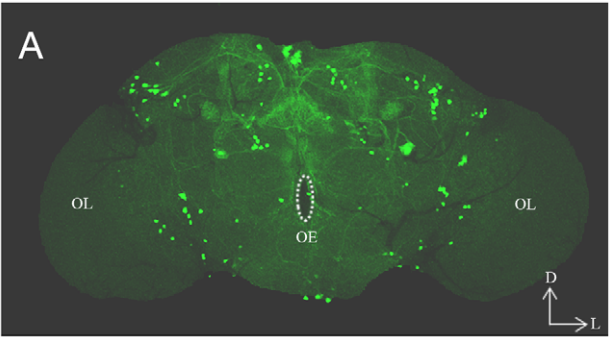
\includegraphics[width=\linewidth]{img/2025_01_15/Ih_expression_drosophila.png}
    \caption{Source: Fig. 3A from \cite{gonzalo-gomezIhCurrentNecessary2012}}
\end{wrapfigure}
In Drosophila, Ih is strongly expressed in compound eyes, second and third segments of antennae \cite{chenFunctionalStudyHyperpolarization2012}

I could not find literature specifially stating that Ih is expressed in R5,
but the image from \cite{gonzalo-gomezIhCurrentNecessary2012} might indicate that
Ih is expressed in ring neurons.

Kinetics of Ih channels in Drosophila are also not fully described in the literature. I found
only two papers on that matter: \cite{gisselmannVariantsDrosophilaMelanogaster2005} and
\cite{ishiiPeripheralCterminalDomains2007}. However, \cite{ishiiPeripheralCterminalDomains2007}
did not specifically described the kinetics of Drosophila Ih currents (DMIH), but introduced DMIH
core region into mamallian Ih channels and studied kinetics of the latter. \cite{gisselmannVariantsDrosophilaMelanogaster2005}
reported parameters for activation of DMIH channels, but provided values of the time constant
only within the test potential range of $[-180, -150]$mV.

\textbf{Simplification}: set the time constant not to depend on membrane potential


\section{Temporal width of the bursts: do we need an additional current?}
    
The voltate at which the Ih channels are activated is below the one of the
T-type channels ($V_{1/2}=-123$mV for the Ih channels, and $\approx-56$mV for T-type
channels). This means, that (given the depolarizing nature of Ih current)
the main function for the Ih channels will be to drive the
membrane potential to the activation threshold for the T-Type channels, after
hyperpolarization deinactivated them. Ih current affects the time between the spikes.

By visual inspection, the temporal width of the bursts of R5 neurons is around
0.3 seconds. The simulation of the T-Type and leak channels shows that the width of the
t-type current when corresponding channels are active is considerably smaller. Thus,
if bursts lay on top of the t-type current, the width of the bursts will be smaller
as well. There are two possibilities solve this.

\textcolor{orange}{
    \textbf{1. Increase deactivation time constant (But, will it be biologically plausible?)}.
}
As the activation/deactivation time constant
is much faster than the ones of inactivation, the width of the t-type current mainly
follows the deactivation of the activation gate

The experiment in the paper providing values for the T-Type channel kinetics 
was done using 10mM Ca concentration. The Ca concentration outside membrane was
set to 0.5mM in the model

I fitted IV relationship of the model to the data by varying shift of the
steady-state activation curve along voltage axis and scale of the activation time
constant. The fits with various initial guesses were around 4.5mV for the shift and
0.5-0.6 for the scale.

To adapt the time constant for the increase in the bursting length the scaling
constant should be not smaller, but larger than 1 (according to simulations of t-type
current, 2-2.5 might suffice). What does the literature say?

\begin{figure}[H]
    \centering
    % First row
    \begin{subfigure}[t]{0.45\textwidth}
        \centering
        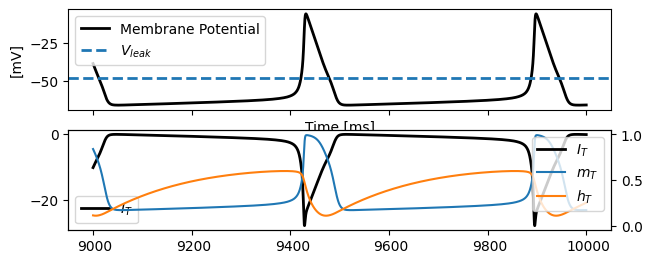
\includegraphics[width=\textwidth]{./img/2025_01_15/simulation_0,5.png}
        \caption{Scaling factor for activation/deactivation time constant - 0.5}
    \end{subfigure}
    \hfill
    \begin{subfigure}[t]{0.45\textwidth}
        \centering
        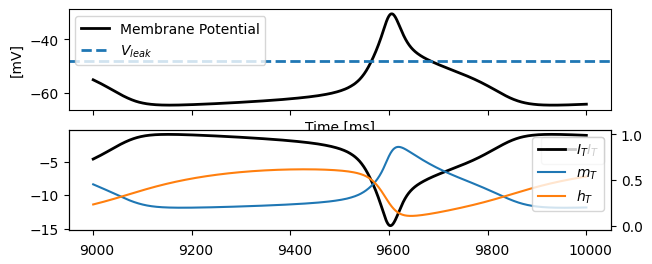
\includegraphics[width=\textwidth]{./img/2025_01_15/simulation_2,5.png}
        \caption{Scaling factor for activation/deactivation time constant - 2.5}
    \end{subfigure}
\end{figure}

There is not much data on Drosophila T-Type channels. However I found two papers
on $Ca_v3.1$ T-Type channels (in humans)

\begin{wrapfigure}[9]{l}{0.4\textwidth}
    \vspace{-1.1\baselineskip}
    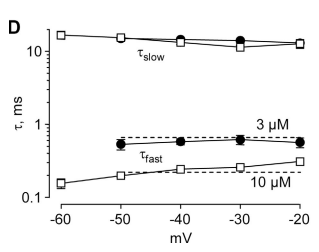
\includegraphics[width=0.4\textwidth]{img/2025_01_15/ca_modul_of_t_type_khan.png}
    \caption{Source: Fig. 3A from \cite{gonzalo-gomezIhCurrentNecessary2012}}
\end{wrapfigure}
1. \cite{khanPermeationGatingCaV312008} fit the tail currents to sum of
two exponentials. The slower component demonstrated $[Ca]_{outside}$ dependent
modulation (activation ???) - increase in amplitude with reduction of $[Ca]_{outside}$, while slower
component did not demonstrate such behavior

2. \cite{talaveraExtracellularCa2Modulates2003} Reported positive
shift of the functions for activation and inactivation time constants. This will
effectively increase the time constant per given test potential (contrary to what
was described in \cite{khanPermeationGatingCaV312008})

\vspace{1.3cm}

\begin{figure}[H]
    \centering
    % First row
    \begin{subfigure}[t]{0.48\textwidth}
        \centering
        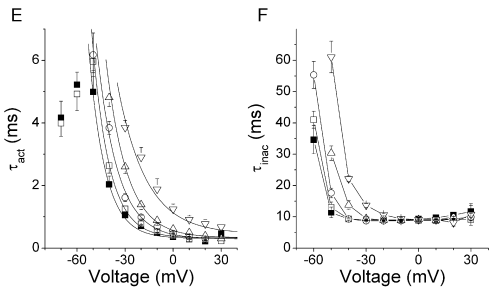
\includegraphics[width=\textwidth]{./img/2025_01_15/ca_modul_of_t_type_talavera_2mm.png}
        \caption{2mM extracellular Ca concentration}
    \end{subfigure}
    \hfill
    \begin{subfigure}[t]{0.48\textwidth}
        \centering
        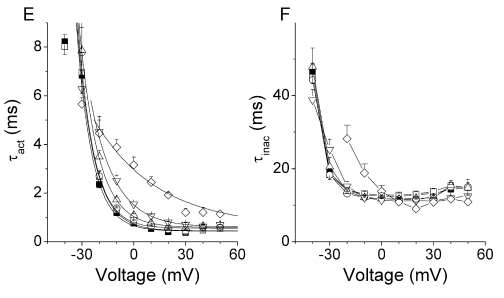
\includegraphics[width=\textwidth]{./img/2025_01_15/ca_modul_of_t_type_talavera_20mm.png}
        \caption{20mM extracellular Ca concentration}
    \end{subfigure}
    \label{fig:data_from_jeong}
    \caption{Source Fig. 1 and 2 in \cite{talaveraExtracellularCa2Modulates2003}}
\end{figure}

\color{red}
\begin{itemize}
    \item Although there is one gene for T-Type ca current, can the gene undergo alternative
    splicing? At least there were papers about alternative splicing of alpha1 subunit.
    Is this subunit common? Or is it different in different channels?
\end{itemize}
\color{black}

\textcolor{orange}{
    \textbf{2. Introduce additional depolarizing current which is activated by the t-type current
(Let us call it channel X and corresponding X current)}
}

\textbf{Idea}: T-Type current activate activate X channels having slow deactivation/inactivation.
The spikes lay on top of the X current (instead of the T-type current).

\textbf{Proposal}: Two gates, activation and inactivation. X channels
are activated at more depolarized states than t-type ones. The inactivation gate
opens at around same potential as the activation of the t-type channel. Furthermore,
deactivation and inactivation should be slow in comparison to the t-type channel.


\color{orange}
\section{Modulation of exitability by T-Type channels}
\color{black}

Experimental finding, that blocking T-Type channels reduces activity in R5 still can be
implemented with single compartment model (at least there is a hope).

\textbf{Possible explanation:} Resting membrane potential of R5 neurons is at around
$-49$mV. Coincidentally, at this membrane potential the steady-state activation ($m^3$)
and inactivation curves intersect. So, at rest there is a depolarizing window-current
through the T-Type channels. This will bias R5 neuron to more excitable states to an extent
when without this bias the visual input cannot drive the membrane potential to the
firing threshold.

\section{Choosing model parameters}

There exist range of parameter values where we see oscillations in T-Type - leak
current without external input. If this is plausible, than the full model might
burst without external input (is this biologically plausible? I think not).

So, to choose the parameters one can introduce two constraints on the parameters:
the system should have a stable fixed points in two cases: 1) When sodium channels
are blocked, and 2) when they are not blocked.

\printbibliography

\end{document}